
\documentclass[letterpaper, 10pt, conference]{ieeeconf}
\usepackage{graphicx}
\overrideIEEEmargins
\usepackage[utf8]{inputenc}
\usepackage[T1]{fontenc}
\usepackage{graphics}
\usepackage{amsmath}
\usepackage{amssymb}
\usepackage{booktabs}

% Spanish names and arabic numbering for tables (ieeeconf already uses Fig. for figures)
\makeatletter
\renewcommand{\fnum@table}{Tabla~\thetable.}
\makeatother
\renewcommand{\thetable}{\arabic{table}}

\title{\LARGE \bf
Clasificaci\'on de Sentimientos de Rese\~nas de Pel\'iculas en IMDb\\
con Redes Neuronales Recurrentes
}

\author{
  Yezid Garcia$^{*}$, Juan Martin Santos$^{*}$, Jaime Rodriguez$^{*}$ \\
  $^{*}$Grupo 24. C\'odigos: 200810710, 202013610, 200717791
}

\begin{document}

\maketitle
\thispagestyle{empty}
\pagestyle{empty}

%%%%%%%%%%%%%%%%%%%%%%%%%%%%%%%%%%%%%%%%%%%%%%%%%%%%%%%%%%%%%%%%%%%%%%%%%%%%%%%%
\section{Introducci\'on}

El an\'alisis de sentimiento es una tarea del procesamiento de lenguaje natural
que determina la polaridad emocional de un texto. En el contexto de rese\~nas
de pel\'iculas, el problema consiste en clasificar autom\'aticamente si una
rese\~na expresa una opini\'on positiva o negativa. Esta capacidad tiene
aplicaci\'on directa en sistemas de recomendaci\'on y monitoreo de reputaci\'on,
donde procesar grandes vol\'umenes de texto de forma manual no es viable.

Los enfoques cl\'asicos basados en frecuencia de t\'erminos ignoran el orden
de las palabras y pierden informaci\'on contextual. Las redes con celdas de
memoria a largo y corto plazo (LSTM) [1] superan esta limitaci\'on al procesar
secuencias de tokens y capturar dependencias entre palabras distantes. La
variante bidireccional (BiLSTM) combina estados ocultos procesados en ambas
direcciones, proporcionando a cada posici\'on acceso al contexto anterior y
posterior. Las representaciones distribucionales de palabras [2] codifican
similitud sem\'antica en vectores densos entrenados sobre grandes corpus;
inicializar un modelo con vectores preentrenados como GloVe [3] mejora la
generalizaci\'on cuando el conjunto de entrenamiento es de tama\~no moderado.

Este trabajo describe la implementaci\'on y evaluaci\'on de un modelo BiLSTM
con embeddings GloVe para la clasificaci\'on binaria de rese\~nas del conjunto
IMDb [4]. Se presentan el pipeline de preprocesamiento, la arquitectura del
modelo, la estrategia de entrenamiento, los resultados cuantitativos y
cualitativos, y un an\'alisis de los factores que explican el comportamiento
del modelo.

%%%%%%%%%%%%%%%%%%%%%%%%%%%%%%%%%%%%%%%%%%%%%%%%%%%%%%%%%%%%%%%%%%%%%%%%%%%%%%%%
\section{Metodolog\'ia}

Para el desarrollo del proyecto se sigui\'o el ciclo tradicional de aprendizaje
autom\'atico: entendimiento del problema, recopilaci\'on y preparaci\'on de los
datos, dise\~no y entrenamiento del modelo, evaluaci\'on sobre un conjunto de
prueba independiente, y an\'alisis de los resultados obtenidos.

El conjunto de datos contiene 40\,000 rese\~nas de IMDb [4] con etiqueta
binaria de sentimiento, balanceado en 20\,000 muestras por clase y sin valores
nulos. La divisi\'on es estratificada por clase: 80\,\% para entrenamiento
(32\,000 muestras), 10\,\% para validaci\'on (4\,000) y 10\,\% para prueba
(4\,000).

Cada rese\~na pasa por un pipeline de cinco pasos: eliminaci\'on de etiquetas
HTML; descarte de caracteres no alfab\'eticos; conversi\'on a min\'usculas;
eliminaci\'on de palabras funcionales en ingl\'es; y lematizaci\'on, que reduce
cada token a su forma can\'onica (\textit{running} $\to$ \textit{run}). El
vocabulario se construye exclusivamente sobre el conjunto de entrenamiento para
evitar fuga de informaci\'on, y las secuencias se rellenan o truncan a 300
tokens.

Los embeddings se inicializan con vectores GloVe de 100 dimensiones [3], con
una cobertura del 77.2\,\% sobre el vocabulario. Siguiendo la estrategia de
ajuste progresivo propuesta en [5], los embeddings se congelan durante las tres
primeras \'epocas para que las capas recurrentes converjan sin distorsionar las
representaciones preentrenadas; a partir de la cuarta \'epoca se descongelan
con una tasa de aprendizaje diez veces menor.

El modelo \textit{SentimentBiLSTM} encadena las capas descritas en la Tabla~1.
La capa BiLSTM de 128 unidades por direcci\'on procesa la secuencia en ambos
sentidos; un promedio sobre todos los estados ocultos (mean pooling) produce
una representaci\'on de longitud fija. Esta operaci\'on, validada en [6], es
superior al uso del \'ultimo estado oculto para secuencias largas donde el
sentimiento est\'a distribuido a lo largo del texto. Una capa lineal con
activaci\'on sigmoide produce la clasificaci\'on final.

\begin{table}[h]
\centering
\caption{Capas del modelo \textit{SentimentBiLSTM}.}
\label{tab:arquitectura}
\resizebox{8.5cm}{!}{
\begin{tabular}{llr}
\toprule
\textbf{Capa} & \textbf{Dimensi\'on de salida} & \textbf{Par\'ametros} \\
\midrule
Embedding GloVe 100d      & $B \times 300 \times 100$ & 7{,}449{,}500 \\
Abandono (p = 0.3)        & $B \times 300 \times 100$ & 0             \\
BiLSTM (128 ud., 1 capa)  & $B \times 300 \times 256$ & 267{,}264     \\
Mean Pooling              & $B \times 256$            & 0             \\
Abandono (p = 0.3)        & $B \times 256$            & 0             \\
Lineal + Sigmoide         & $B \times 1$              & 257           \\
\midrule
\textbf{Total}            &                           & \textbf{7{,}685{,}277} \\
\bottomrule
\end{tabular}}
\end{table}

El entrenamiento usa Adam con tasa de aprendizaje inicial de $10^{-3}$ y
p\'erdida de entrop\'ia cruzada binaria, con lotes de 128 muestras. Se
aplican tres mecanismos de control: un planificador que reduce la tasa de
aprendizaje a la mitad si la p\'erdida de validaci\'on no mejora en dos
\'epocas consecutivas; limitaci\'on de la norma del gradiente a 1.0, que [7]
identifica como cr\'itico para estabilizar el entrenamiento de LSTM en
secuencias largas; y parada anticipada con paciencia de cinco \'epocas. Las
m\'etricas de evaluaci\'on son precisi\'on, recall y F1-score, calculadas
sobre el conjunto de prueba al finalizar el entrenamiento.

%%%%%%%%%%%%%%%%%%%%%%%%%%%%%%%%%%%%%%%%%%%%%%%%%%%%%%%%%%%%%%%%%%%%%%%%%%%%%%%%
\section{Resultados}

Se implement\'o un clasificador de sentimiento binario sobre 40\,000 rese\~nas
de IMDb, entrenando una red BiLSTM de una capa con embeddings GloVe de 100
dimensiones inicializados desde vectores preentrenados y ajustados de forma
progresiva. A continuaci\'on se presentan los resultados mas relevantes.

\subsection{Resultados cuantitativos}

Se entren\'o el modelo durante un m\'aximo de 20 \'epocas con parada
anticipada activada en la \'epoca 19. La Fig.~1 muestra la evoluci\'on de
la p\'erdida en entrenamiento y validaci\'on, y las m\'etricas de precisi\'on,
recall y F1 en validaci\'on por \'epoca.

\begin{figure}[h]
  \centering
  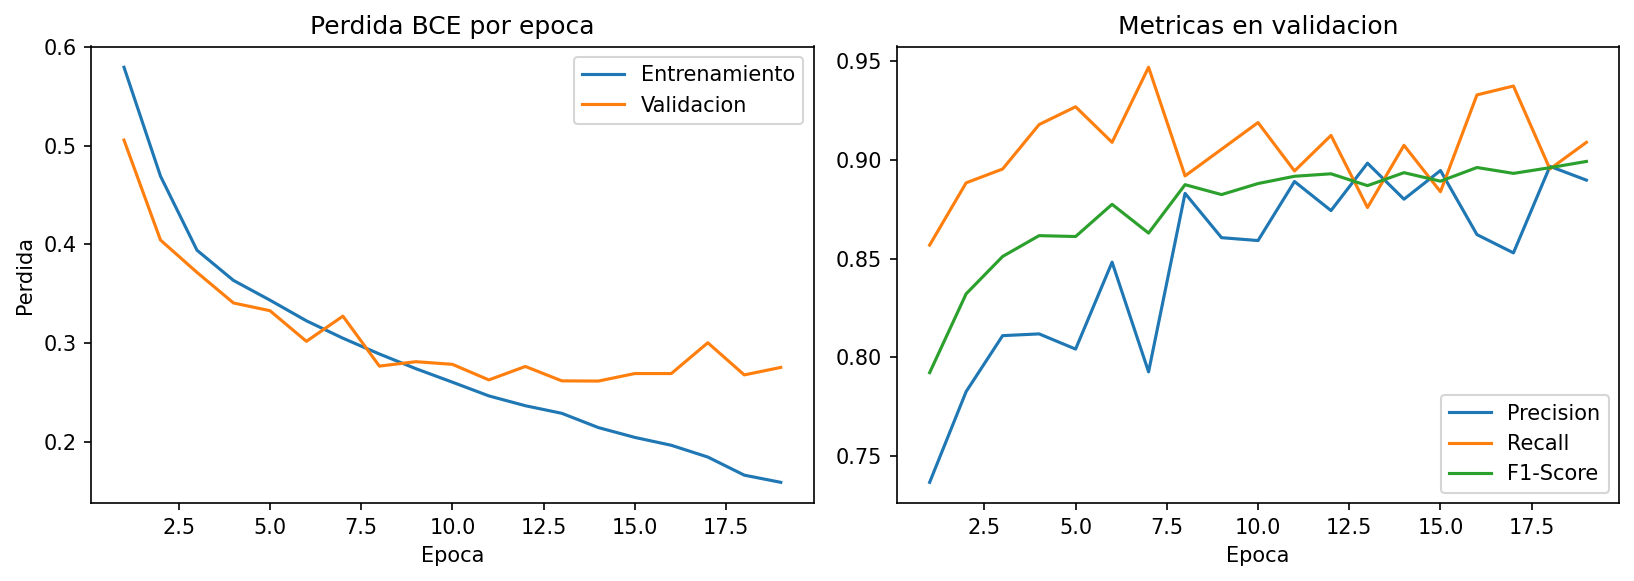
\includegraphics[width=0.98\linewidth]{curvas_entrenamiento.png}
  \caption{P\'erdida BCE (izq.) y m\'etricas de validaci\'on (der.) por
  \'epoca. Parada anticipada en \'epoca 19.}
  \label{fig:curvas}
\end{figure}

La Tabla~2 compara las m\'etricas de validaci\'on en cuatro momentos del
entrenamiento para cuantificar el efecto de cada fase: con embeddings
congelados (\'ep.~3), al inicio del ajuste fino (\'ep.~6), en la convergencia
(\'ep.~11) y en la \'ultima \'epoca ejecutada (\'ep.~19). La Tabla~3 reporta
los resultados finales sobre el conjunto de prueba.

\begin{table}[h]
\centering
\caption{M\'etricas de validaci\'on por fase de entrenamiento.}
\label{tab:evolucion}
\resizebox{8.5cm}{!}{
\begin{tabular}{lccc}
\toprule
\textbf{Fase} & \textbf{Precisi\'on} & \textbf{Recall} & \textbf{F1} \\
\midrule
\'Ep.~3 --- embeddings congelados  & 0.811 & 0.895 & 0.851 \\
\'Ep.~6 --- inicio ajuste fino     & 0.848 & 0.909 & 0.878 \\
\'Ep.~11 --- convergencia          & 0.889 & 0.894 & 0.892 \\
\'Ep.~19 --- parada anticipada     & 0.890 & 0.909 & 0.899 \\
\bottomrule
\end{tabular}}
\end{table}

\begin{table}[h]
\centering
\caption{M\'etricas finales sobre el conjunto de prueba (4\,000 muestras).}
\label{tab:prueba}
\begin{tabular}{lc}
\toprule
\textbf{M\'etrica} & \textbf{Valor} \\
\midrule
Precisi\'on  & 0.877 \\
Recall       & 0.910 \\
F1-Score     & \textbf{0.893} \\
\bottomrule
\end{tabular}
\end{table}

\subsection{Resultados cualitativos}

El recall supera sistem\'aticamente a la precisi\'on tanto en validaci\'on como
en prueba (0.910 frente a 0.877). Esto indica una tendencia del modelo a
clasificar como positivo ante la ambig\"uedad, comportamiento consistente con
el sesgo de los vectores GloVe: intensificadores frecuentes en rese\~nas como
\textit{amazing} o \textit{terrible} tienen carga emocional pronunciada que el
modelo asocia con la clase positiva incluso en contextos negativos. El efecto
se mantiene estable tras el ajuste fino.

La convergencia es r\'apida en las primeras seis \'epocas, donde el F1 pasa
de 0.792 a 0.878; las \'epocas posteriores aportan mejoras marginales (0.878
a 0.899). La brecha creciente entre la p\'erdida de entrenamiento y la de
validaci\'on a partir de la \'epoca 11 indica sobreajuste moderado que la
parada anticipada contiene sin eliminarlo por completo.

%%%%%%%%%%%%%%%%%%%%%%%%%%%%%%%%%%%%%%%%%%%%%%%%%%%%%%%%%%%%%%%%%%%%%%%%%%%%%%%%
\section{Discusi\'on}

El F1 de 0.893 sobre el conjunto de prueba es consistente con los rangos
reportados para arquitecturas recurrentes sobre IMDb en [5]. El resultado
corresponde al rango esperado para una sola capa BiLSTM: [7] muestra que
capas adicionales no garantizan mejoras en clasificaci\'on de secuencias de
longitud moderada y pueden introducir inestabilidad. El mean pooling sobre los
estados ocultos, validado en [6], produce representaciones m\'as estables que
el \'ultimo estado oculto para rese\~nas largas donde el sentimiento est\'a
distribuido a lo largo del texto, lo que contribuye a la consistencia de las
m\'etricas en las \'epocas finales.

La estrategia de congelado y ajuste fino es efectiva: la Tabla~2 muestra una
ganancia de 2.7 puntos de F1 entre la \'ep.~3 y la \'ep.~6, resultado
coherente con [8], que demuestra que los embeddings ajustables superan a los
est\'aticos en tareas de clasificaci\'on de texto. El ajuste fino con tasa de
aprendizaje reducida preserva las representaciones sem\'anticas preentrenadas
mientras el modelo incorpora patrones espec\'ificos del dominio. La cobertura
de 77.2\,\% de GloVe es suficiente para aportar informaci\'on sem\'antica
\'util desde las primeras \'epocas; el 22.8\,\% restante, inicializado en
cero, corresponde principalmente a t\'erminos especializados o nombres propios
de pel\'iculas con menor impacto en la clasificaci\'on.

Entre las limitaciones del trabajo, el n\'umero de \'epocas de congelado es
fijo y no se adapta a la velocidad de convergencia de cada ejecuci\'on. Las
rese\~nas con m\'as de 300 tokens se truncan, perdiendo el contexto del final
del texto, donde el cr\'itico frecuentemente expresa su valoraci\'on definitiva.
Adicionalmente, no se realiz\'o b\'usqueda sistem\'atica de hiperpar\'ametros,
por lo que configuraciones alternativas podr\'ian mejorar el rendimiento. Como
trabajo futuro, resulta de inter\'es explorar mecanismos de atenci\'on sobre
los estados del BiLSTM como alternativa al mean pooling, evaluar el impacto de
distintas duraciones de la fase de congelado y comparar el modelo con
arquitecturas Transformer ligeras aplicadas al mismo conjunto de datos.

%%%%%%%%%%%%%%%%%%%%%%%%%%%%%%%%%%%%%%%%%%%%%%%%%%%%%%%%%%%%%%%%%%%%%%%%%%%%%%%%
\clearpage

\begin{thebibliography}{99}

\bibitem{hochreiter1997}
S.~Hochreiter and J.~Schmidhuber,
``Long short-term memory,''
\textit{Neural Computation}, vol.~9, no.~8, pp.~1735--1780, 1997.

\bibitem{mikolov2013}
T.~Mikolov, K.~Chen, G.~Corrado, and J.~Dean,
``Efficient estimation of word representations in vector space,''
\textit{arXiv preprint arXiv:1301.3781}, 2013.

\bibitem{pennington2014}
J.~Pennington, R.~Socher, and C.~D.~Manning,
``GloVe: Global vectors for word representation,''
in \textit{Proc. EMNLP}, pp.~1532--1543, 2014.

\bibitem{maas2011}
A.~L.~Maas, R.~E.~Daly, P.~T.~Pham, D.~Huang, A.~Y.~Ng, and C.~Potts,
``Learning word vectors for sentiment analysis,''
in \textit{Proc. 49th Annual Meeting of the ACL}, pp.~142--150, 2011.

\bibitem{howard2018}
J.~Howard and S.~Ruder,
``Universal language model fine-tuning for text classification,''
in \textit{Proc. ACL}, pp.~328--339, 2018.

\bibitem{conneau2017}
A.~Conneau, D.~Kiela, H.~Schwenk, L.~Barrault, and A.~Bordes,
``Supervised learning of universal sentence representations from natural
language inference data,''
in \textit{Proc. EMNLP}, pp.~670--680, 2017.

\bibitem{greff2017}
K.~Greff, R.~K.~Srivastava, J.~Kout\'nik, B.~R.~Steunebrink, and J.~Schmidhuber,
``LSTM: A search space odyssey,''
\textit{IEEE Trans. Neural Netw. Learn. Syst.}, vol.~28, no.~10,
pp.~2222--2232, 2017.

\bibitem{kim2014}
Y.~Kim,
``Convolutional neural networks for sentence classification,''
in \textit{Proc. EMNLP}, pp.~1746--1751, 2014.

\end{thebibliography}

\end{document}
